\input{~/macro.tex}
\title{%定常的とみなせる外力が加わった際の荷電粒子の運動
}
\author{%20B01392 松本侑真
}
\date{\today}
\begin{document}
\maketitle
\begin{abstract}
	プラズマ物理学において、定常的な外力が加わった差異の荷電粒子の運動についてまとめる。
	また、外力が時間的に変化している場合においても、粒子のサイクロトロン運動よりも十分にゆっくりであれば成立する。
\end{abstract}
\tableofcontents
\newpage

\section{一様定常磁場と定常的な外力}
荷電粒子に対して一様定常磁場$\bm{B}$と定常的な外力$\bm{F}(\bm{x})$が印加している場合を考える。
まずは、粒子の速度ベクトルを磁場$\bm{B}$に垂直な方向と平行な方向へと分解する:
\begin{equation}
	\bm{v} = \bm{v}_{\perp} + \bm{v}_{\varParallel}\;。
\end{equation}
外力の磁場に平行な成分については、大きさが$\bm{F}_{\varParallel}/m$の等加速度直線運動を与えるだけである。
そのため、以下では磁場$\bm{B}$と垂直な成分のみを考える($\bm{F} = \bm{F}_{\perp}$)。このとき、磁場に垂直な方向における荷電粒子の運動方程式は
\begin{equation}
	m\dot{\bm{v}}_{\perp} = q\qty(\bm{v}_{\perp}\cross\bm{B}) + \bm{F}_{\perp}
	\label{eq:mv_all}
\end{equation}
となる。外力が加わっていない場合、磁場$\bm{B}$に垂直な方向において荷電粒子は円運動を行うことが直ちにわかる。そのため、$\bm{v}_{\perp}$を$\bm{v}_0$(円運動成分)と$\bm{v}_{\text{F}}$(ドリフト運動成分)に分解して考える。
\footnote{ローレンツ力と外力が張る平面が磁場と垂直であるため、$\bm{v}_{\varParallel}$方向に$\bm{v}_{\text{F}}$は存在しない。}
このとき、円運動成分については以下の運動方程式が成立している:
\begin{equation}
	m\dot{\bm{v}}_0 = q\qty(\bm{v}_0\cross\bm{B})\;。
\end{equation}
定常的な外力が印加されていることから、$\bm{v}_{\text{F}}$の時間変化がないと考えて良い
\footnote{円運動について平均を取ると直流成分のみが残り、それが$\bm{v}_{\text{F}}$となるはずだから時間変化はないと考えて良い。

\noindent
より正確には、円運動の周波数$\omega_{\text{c}}$より緩やかに時間変化をする場合であれば適用できる:
\begin{equation}
	\omega_{\text{c}} \gg \qty|\pdv{\bm{F}_{\perp}}{t}\bigg/\bm{F}_{\perp}|\;。
\end{equation}
}ため、
式\eqref{eq:mv_all}は
\begin{equation}
	m\dot{\bm{v}}_0 = q\qty(\bm{v}_0\cross\bm{B}) + q\qty(\bm{v}_{\text{F}}\cross\bm{B}) + \bm{F}_{\perp}
\end{equation}
と書き直すことができる。したがって、
\begin{equation}
	q\qty(\bm{v}_{\text{F}}\cross\bm{B}) + \bm{F}_{\perp} = \bm{0}
\end{equation}
が成立している。右から$\bm{B}$の外積を取ってみると、$(\bm{a}\cross \bm{b})\cross \bm{c} = (\bm{a}\cdot \bm{c})\bm{b} - (\bm{b}\cdot \bm{c})\bm{a}$を用いて、
\begin{equation}
	q\qty(\bm{v}_{\text{F}}\cross\bm{B})\cross\bm{B} = -qB^2\bm{v}_{\text{F}} = -\bm{F}_{\perp}\cross\bm{B}
\end{equation}
となる。したがって、ドリフト運動$\bm{v}_{\text{F}}$は
\begin{equation}
	\bm{v}_{\text{F}} = \frac{\bm{F}_{\perp}\cross\bm{B}}{qB^2} = \frac{\bm{F}\cross\bm{B}}{qB^2}
	\label{eq:drift}
\end{equation}
と求まる。つまり、定常的な外力が加わっている方向には運動しない。
\subsection{定常的な電場が印加されているとき}
例として定常的な電場$\bm{E}$が印加されている場合には、ドリフト運動は電荷に依らないことがわかる。
式\eqref{eq:drift}によると、
\begin{equation}
	\bm{v}_{\bm{E}} = \frac{\bm{E}\cross\bm{B}}{B^2}
\end{equation}
となるため、プラズマ中の電子とイオンは同じ速度で同じ方向にドリフトする。そのため、プラズマ中に電離が生じることがなく、電流は流れない。
また、プラズマ全体は磁力線を横切ってドリフトしていくことがわかる。

\newpage
\section{空間的に変化する定常磁場}
\subsection{磁場と垂直な方向に勾配が生じている場合}
次に、磁場が空間的に変化する場合を考えよう。磁場$\bm{B}$は$z$成分のみを持つするとして、その強さが$y$依存性を持つとする:
\begin{equation}
	\bm{B} =
	\begin{pmatrix}
		0 & 0 & B(y)
	\end{pmatrix}^\top\;。
\end{equation}
\begin{figure}[H]
	\centering
	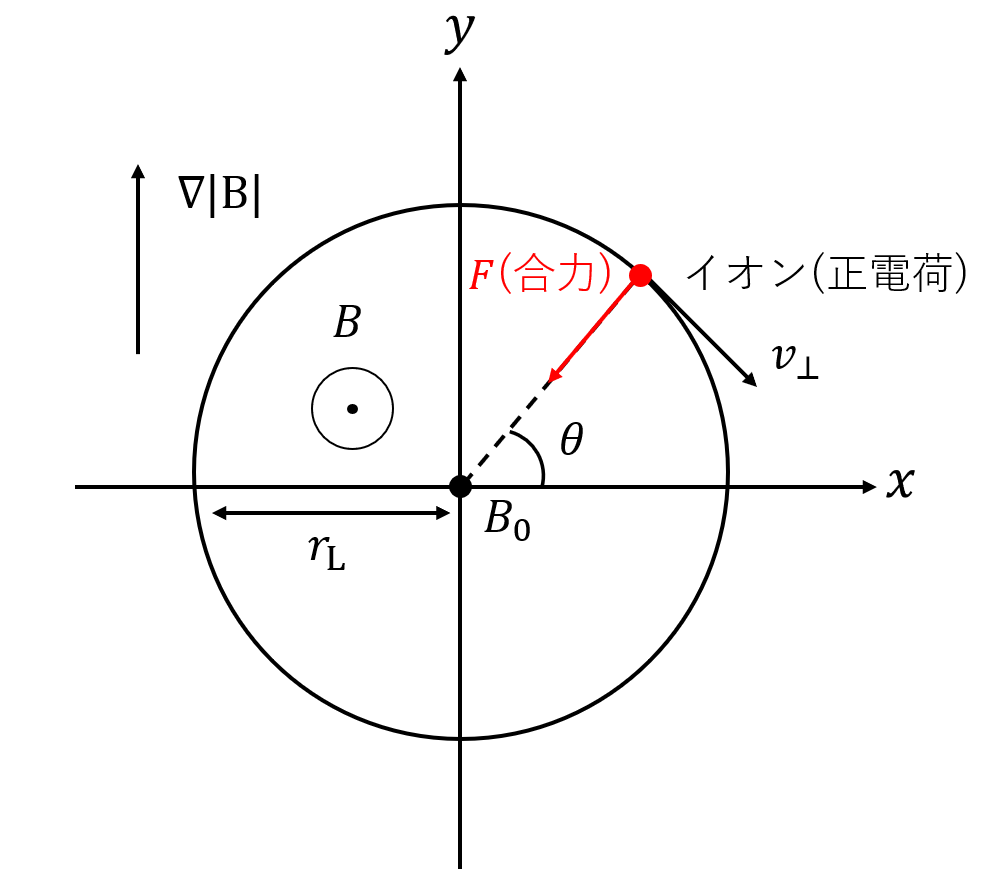
\includegraphics[width=0.6\linewidth]{gradB.png}
	\caption{磁場と垂直な方向に勾配が生じている場合}
	\label{fig:gradB}
\end{figure}
また、$B(y)$は緩やかに変化しているとする。
\footnote{
	緩やかさを表す指標としては、特性長$L$という概念を考えれば良い。
	これは、ある物理量の変化が物理量自体に影響を及ぼすのに必要な距離の目安であり、今の状況であれば
	\begin{equation}
		L \coloneqq B_0/(\partial_yB_0)
	\end{equation}
	である。円運動の半径が急激に変化しない場合を考えたいため、
	$L\gg r_{\text{L}}$が成立しているとき、$B(y)$は緩やかに変かしていると言える。
}
すなわち、回転中心におけるTaylor展開の1次項までで近似できるとする:
\begin{equation}
	B(y) = B_0 + \qty(\pdv{B}{y})_0y = B_0 + \qty(\pdv{B}{y})_0r_{\text{L}}\sin\theta\;。
\end{equation}
ここで、$r_{\text{L}}$はLarmor半径であり、大きさ$B$の定常磁場のみが印加されている際の粒子の磁場に直交する速度成分の大きさを$v_{\perp}$として、$r_{\text{L}} = mv_{\perp}/qB$と表される。
また、回転中心における磁場の大きさを$B_0$とした。さらに、粒子が1旋回する間では磁場の変化が微小であると仮定しているため、$y = r_{\text{L}}\sin\theta$が成立している。
粒子にかかる力について、1旋回に関する平均値を取るとLarmor円運動に関する成分は$0$になるため、磁場の変化によって生じる成分が残る。これを定常的な外力$\bm{F}$とみなすこととする。
1旋回中のイオンにかかるLorentz力を考える。$v_x = v_{\perp}\cos\theta,\,v_y = -v_{\perp}\sin\theta$であることに注意すると、$F_x,\,F_y$は以下のように計算できる:
\begin{align}
	F_x & = qv_yB_z = -qv_{\perp}\cos\theta B(y) = -qv_{\perp}\cos\theta\qty(B_0 + \qty(\pdv{B}{y})_0r_{\text{L}}\sin\theta)\;,  \\
	F_y & = -qv_xB_z = -qv_{\perp}\sin\theta B(y) = -qv_{\perp}\sin\theta\qty(B_0 + \qty(\pdv{B}{y})_0r_{\text{L}}\sin\theta)\;。
\end{align}
したがって、$\bar{F}_x = 0,\,\bar{F}_y \neq 0$となることがわかる。実際に計算すると、
\begin{equation}
	\bar{F}_y = -qv_{\perp}r_{\text{L}}\qty(\pdv{B}{y})_0\frac{1}{2\pi}\int_0^{2\pi}\sin^2\theta\dd{\theta}
	= -\frac{1}{2}qv_{\perp}r_{\text{L}}\qty(\pdv{B}{y})_0 = -\frac{mv^2_{\perp}/2}{B_0}\qty(\pdv{B}{y})_0
\end{equation}
となるため、磁気モーメント$\mu_m \coloneqq mv^2_{\perp}/(2B)$を用いて、一定の外力$F_y = -\mu_m\qty(\pdv*{B}{y})$がイオンの運動中に印加されていると考えて良いことがわかる。
磁場に垂直な一般の方向に対する変化に拡張するのは容易であり、
\begin{equation}
	\bm{F} = -\mu_m\qty(\grad{B})_{\perp}
\end{equation}
と表される。なお、磁気モーメントとは、電流が旋回しているときの面積と電流の積であるため、
\begin{equation}
	\mu_m = SI = \pi r_{\text{L}}^2\times q\qty(\frac{\omega_c}{2\pi}) = \qty(r_{\text{L}}\omega_c)^2\frac{m}{qB}\frac{q}{2} = \frac{mv_{\perp}^2/2}{B}
\end{equation}
のようにして求められる値である。
話を戻して、磁場の垂直方向の勾配によって生じる外力のドリフト速度は
\begin{equation}
	\bm{v}_{B} = \frac{-\mu_m\qty(\grad{B})_{\perp}\cross\bm{B}}{qB^2} = \frac{\mu_m\bm{B}\cross\grad{B}}{qB^2}
\end{equation}
となる。これをgradBドリフトと呼ぶ。
\subsection{湾曲磁場について}
次に、磁場が湾曲している場合について考える。荷電粒子は磁力線の周りをらせん運動するため、磁場が湾曲している場合は遠心力が生じることがわかる。
磁場の曲率半径を$R_\text{c}$として、曲率中心から荷電粒子の位置へ伸びるベクトルを$\bm{R}_{\text{c}}$とする。
このとき、荷電粒子にかかる遠心力$\bm{F}_{cf}$は
\begin{equation}
	\bm{F}_{cf} = \frac{m\bm{v}^2_{\varParallel}}{R_{\text{c}}}\frac{\bm{R}_{\text{c}}}{R_{\text{c}}}
\end{equation}
となる。ただし、$\bm{v}_{\varParallel}$は磁力線と平行な方向の荷電粒子の速度ベクトルである。
したがって、湾曲磁場によって速度
\begin{equation}
	\bm{v}_{R} = \frac{\bm{F}_{cf}\cross\bm{B}}{qB^2} = \frac{mv^2_{\varParallel}}{q}\frac{\bm{R}_{\text{c}}\cross\bm{B}}{R_{\text{c}}^2B^2}
\end{equation}
のドリフト運動が生じることがわかる。このドリフトは湾曲ドリフトや遠心力ドリフトと呼ばれる。
さらに、湾曲ドリフトが生じていれば必ずgradBドリフトが存在することがわかる。
磁場が湾曲している場合、局所的には円形に湾曲していると考えられる。
ここで、外部電場と外部電流が存在しないことから、$\curl{\bm{B}} = \bm{0}$が成立していることに着目する。
円筒座標系で書き下すと$\bm{B}$が$\theta$成分しか持たないことと、$\bm{B}$は$r$方向にしか変化しないことに注意すると、
\begin{equation}
	\curl{\bm{B}} = \frac{1}{r}\pdv{r}\qty(rB_{\theta})\bm{e}_z = 0\qquad\therefore B_\theta \propto \frac{1}{r}
\end{equation}
が成立する。すなわち、曲率半径$R_{\text{c}}$の近傍では
\begin{equation}
	\qty(\grad{B})_{\perp} = \grad{B} \propto -\frac{\bm{e}_r}{R_{c}^2},\quad\frac{\grad{B}}{B} = -\frac{\bm{R}_{\text{c}}}{R_{\text{c}}^2}
\end{equation}
となる。したがって、gradBドリフトは
\begin{equation}
	\bm{v}_{B} = -\frac{mv^2_{\perp}}{2B}\frac{\grad{B}\cross\bm{B}}{qB^2}
	= \frac{mv^2_{\perp}/2}{q}\frac{\bm{R}_{\text{c}}\cross\bm{B}}{R_{\text{c}}^2B^2}
\end{equation}
が生じる。以上より、湾曲磁場が存在している場合に生じるドリフト速度$\bm{v}_{D}$は
\begin{equation}
	\bm{v}_{D} = \bm{v}_{R} + \bm{v}_{B} = \frac{m}{q}\frac{\bm{R}_{\text{c}}\cross\bm{B}}{R_{\text{c}}^2B^2}\qty(v^2_{\varParallel} + \frac{1}{2}v^2_{\perp})
\end{equation}
となる。このようなドリフトが加わるのは望ましいことではない。
なぜなら、熱核融合プラズマを閉じ込める目的で磁場をトーラス状に曲げた際に、粒子はトーラスの外部にドリフトしてしまうからである。

\subsection{磁場と平行な方向に勾配が生じている場合}
磁場と平行な方向に勾配が生じている場合について考える。
磁場に垂直な方向に勾配が生じている場合は、磁場の方向と垂直な方向へドリフトすることがわかったが、平行な勾配に関してはどうであろうか。
結論から述べると、ドリフト運動は生じない。これは、$\grad{B}\varParallel \bm{B}$が成立しているため、
$\bm{F}\cross\bm{B} = \bm{0}$となることからわかる。しかし、実際に$\bm{F}$の表式を計算してみると面白い結果が得られることを示す。

\begin{figure}[H]
	\centering
	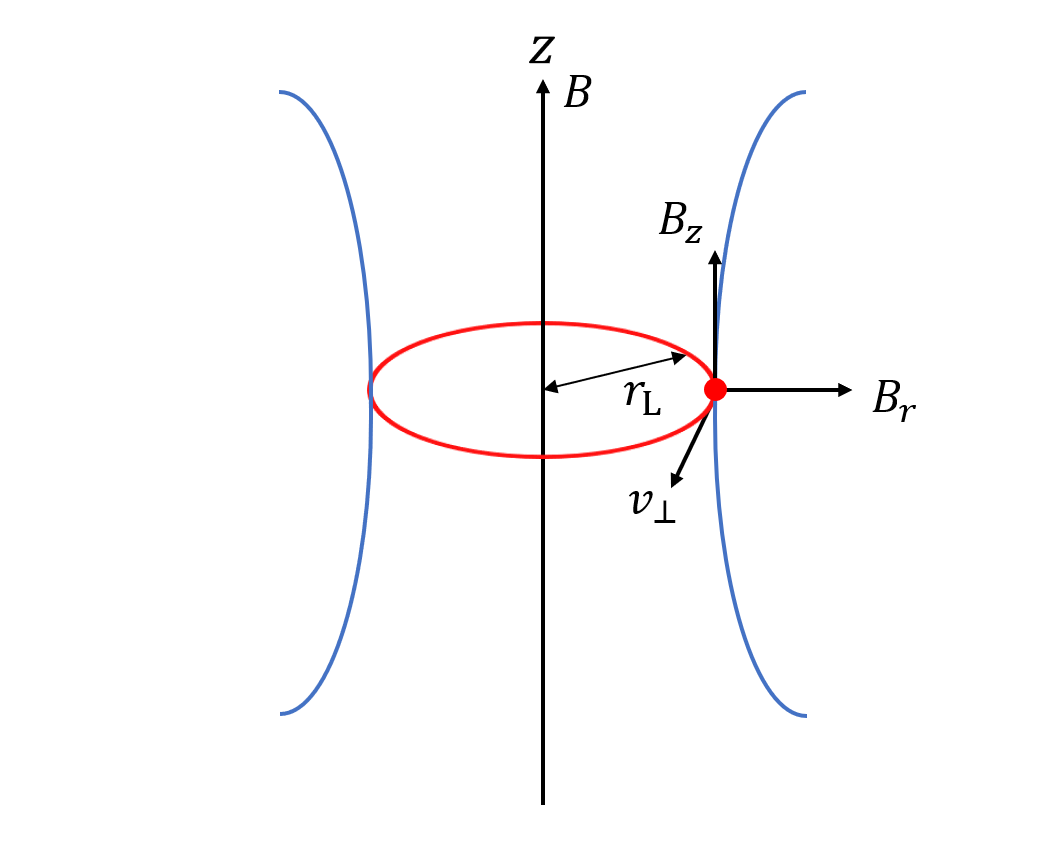
\includegraphics[width=0.5\linewidth]{parallel_B.png}
	\caption{磁場と平行な方向に勾配が生じている場合}
	\label{fig:parallel_B}
\end{figure}
図\ref{fig:parallel_B}のように、磁場のだいたいの向きが$z$方向であり、磁場の強さの変化が$z$方向であるとする。このとき、必然的に磁場の収束・発散により$r$方向にも磁場は存在する。
軸対称性を課すことによって$\theta$方向の磁場は存在しない。
ここでは、Maxwell方程式$\div{\bm{B}} = 0$に着目する。円筒座標系で書き下してみると、
\begin{equation}
	\frac{1}{r}\pdv{r}\qty(rB_r) + \frac{1}{r}\pdv{B_\theta}{\theta} + \pdv{B_z}{z} = 0 \quad\Longrightarrow\quad \pdv{B_r}{r} + \frac{B_r}{r} + \pdv{B_z}{z} = 0
	\label{eq:divB=0}
\end{equation}
となる。$B_r(0) = 0$とすると、$\qty(\pdv*{B_r}{r})_{r\to 0} = \qty(B_r/r)_{r\to 0}$が成立するため、
式\eqref{eq:divB=0}を$B_r$について解くと、$r_{\text{L}}$が十分に小さいときは
\begin{equation}
	B_r(r_{\text{L}}) = -\frac{r_{\text{L}}}{2}\qty(\pdv{B_z}{z})_{r\to 0}
\end{equation}
となる。ここで、旋回中の平均Lorentz力を考えると、$r$方向は$0$となるが、$\bm{B}$と平行な方向の力$F_{\varParallel}$は
\begin{equation}
	F_{\varParallel} = qv_{\perp}B_r(r_{\text{L}})
\end{equation}
となる。したがって、外力$\bm{F} = F_{\varParallel}\bm{e}_z$が荷電粒子にかかる。$r_{\text{L}} = mv_{\perp}/(qB_z)$であることより、
\begin{equation}
	F_{\varParallel} = -\frac{mv^2_{\perp}/2}{B_z}\qty(\pdv{B_z}{z})_{r\to 0}\bm{e}_z = -\mu_{m}\qty(\grad{B})_{\varParallel}
\end{equation}
と計算できる。すなわち、ドリフト運動は生じないが、磁場が弱くなる方向へ荷電粒子が押し出されることがわかる。

\subsection{断熱不変量とその応用例について}
断熱不変量とは、サイクル運動の1周期あたりの物理量などの環境変化が小さいときに一定に保たれる量のことである。ここでは、磁場と平行な方向に勾配が生じている場合に磁気モーメント$\mu_m$が断熱不変量となることを示す。
磁場方向の運動方程式は
\begin{equation}
	m\dv{\bm{v}_{\varParallel}}{t} = -\mu_m\grad B
\end{equation}
となるため、$\bm{v}_{\varParallel}$との内積を考えると次のように計算できる:
\begin{equation}
	\dv{t}\qty(\frac{1}{2}mv_{\varParallel}^2) = -\mu_m\bm{v}_{\varParallel}\cdot\grad B = -\mu_m\dv{B}{t}\;。
	\label{eq:para_hozon}
\end{equation}
磁場は荷電粒子に仕事をしない\footnote{磁場の勾配が円運動に対して十分に緩やかであるため、荷電粒子にはローレンツ力のみが作用すると考えて良い。}ため、
運動エネルギーが一定であることと、$\mu_m = mv_{\perp}^2/(2B)$を用いると、
\begin{equation}
	\dv{t}\qty(\frac{1}{2}mv_{\varParallel}^2) = -\dv{t}\qty(\frac{1}{2}mv_{\perp}^2) = -\dv{t}\qty(\mu_mB)
\end{equation}
となる。式\eqref{eq:para_hozon}を用いることで、
\begin{equation}
	\dv{\mu_m}{t} = 0
\end{equation}
を得る。したがって、磁気モーメント$\mu_m$は断熱不変量である。

次に、磁気ミラーによるプラズマ閉じ込めが上手くいかないことを断熱不変量を用いて示す。
熱運動によって荷電粒子が弱磁場領域から強磁場領域へ動いたとき、粒子は弱磁場方向へ押し戻される方向に力を受ける。
そのため、荷電粒子の集合であるプラズマは磁気ミラーによって封じ込めることが可能と思われるが、実は完全に封じ込めることはできない。

たとえば、$\bm{v}_{\perp} = 0$の場合には磁気モーメントが存在しないため、磁場に沿った方向に力を受けない。
それだけではなく、有限な磁気モーメントを持った荷電粒子に対しても封じ込めが失敗する場合が存在する。
どのような場合に封じ込めが失敗するかについて考察する。
\begin{figure}[H]
	\centering
	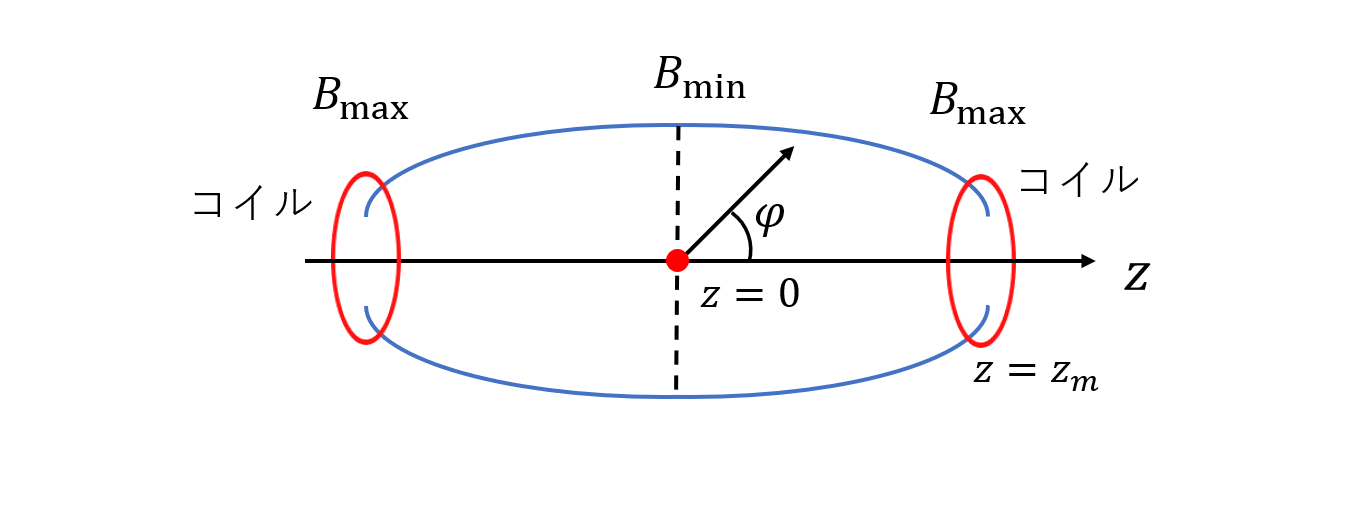
\includegraphics[width=0.8\linewidth]{mirror.png}
	\caption{磁気ミラーによるプラズマ閉じ込めのセットアップ}
	\label{fig:mirror}
\end{figure}
図\ref{fig:mirror}のようなセットアップを考える。$z$軸方向に一様な外部磁場が印加されており、$z=\pm z_m$に円形コイルが置かれている。
円形コイルによって磁場が湾曲されるため、磁束密度の大きさは$z=z_m$で最大値$B_{\text{max}}$を取り、$z=0$で最小値$B_{\text{min}}$を取る。
$z=0$に存在する荷電粒子が$z$軸からの角度$\varphi$で初速度速度$\bm{v} = \bm{v}_{\varParallel} + \bm{v}_{\perp}$を持って運動するとする。
磁場は$z$軸に対する回転対称性により、その勾配は磁場に平行な方向にのみ存在することに注意する($B = B(z)$)。
このとき、粒子が$z=z_m$においても反射されない臨界角度$\varphi_c$が存在することを示す。

そもそも粒子が$z=z_m$で反射される場合、反射点での粒子速度は$\bm{v}_{\varParallel} = \bm{0},\,\bm{v}_{\perp} = \bm{v}$にならないといけない。
そのため、$z=0,\,z_m$における運動エネルギー保存則により、
\begin{equation}
	\frac{1}{2}m\qty( v_{\varParallel}^2 + v^2_{\perp}) = \frac{1}{2}mv^2
\end{equation}
が成立する。さらに、磁気モーメントが断熱不変量となっているため、$z=0,\,z_m$における磁気モーメントが等しいことから
\begin{equation}
	\frac{m\qty(v\sin\varphi_c)^2}{2B_{\text{min}}} = \frac{mv^2}{2B_{\text{max}}}
\end{equation}
が成立する。すなわち、臨界角$\varphi_c$は
\begin{equation}
	\sin^2\varphi_c = \frac{B_{\text{min}}}{B_{\text{max}}}
\end{equation}
と求められる。仮に粒子が反射されない場合、$z=z_m$における粒子の速度は$\bm{v}_{\perp} < \bm{v}$が成立している。したがって、このときの射出角度を$\varphi$とおくと
\begin{equation}
	\sin^2\varphi < \frac{B_{\text{min}}}{B_{\text{max}}} = \sin^2\varphi_c
\end{equation}
が成立する。したがって、臨界角度以下で射出された荷電粒子は$\abs{z} \leq z_m$に閉じ込めることができない。
\footnote{$\varphi = \SI{90}{\degree}$の場合を考えると明らかに荷電粒子は$z=0$上を運動するため、閉じ込め可能な射出角度の不等号の向きを間違えることはない。}
また、このときの磁場の強さの比$B_{\text{min}}/B_{\text{max}}$をミラー比と呼ぶ。

\section{一様定常磁場と時間的に緩やかに変化する一様電場}
電場$\bm{E}$が時間的に定常な場合、ドリフト運動は$\bm{v}_E = E/B$であった。すなわち、イオンと電子はともに同じ速度でドリフトする。
電場$\bm{E}$が時間的に緩やかな変化をする場合、ドリフト速度$\bm{v}_E$も変化するため、粒子には$-m\dot{\bm{v}}_E$の慣性力が作用する。
したがって、新たな外力ドリフトが生じる。粒子の旋回の周波数よりも電場$\bm{E}$の各周波数が十分に小さな場合、$\bm{F}\cross{\bm{B}}$ドリフトの表式を用いることができるため、
\begin{equation}
	\dot{\bm{v}}_E = \frac{\dot{\bm{E}}\cross\bm{B}}{B^2}
\end{equation}
と表すことができる。したがって、慣性力によるドリフト速度$\bm{v}_\text{P}$は
\begin{equation}
	\bm{v}_\text{P} = \frac{-m\dot{\bm{v}}_E\cross\bm{B}}{qB^2} = -\frac{m}{qB^2}\frac{\dot{\bm{E}}\cross\bm{B}}{B^2}\cross\bm{B}
	= \frac{m}{qB^2}\dv{\bm{E}}{t} = \pm\frac{1}{\omega_cB}\dv{\bm{E}}{t}
\end{equation}
と計算できる。このドリフトを分極ドリフトと呼ぶ。
分極ドリフトの特徴としては、$\bm{E}$に平行で$q,\,m$に依存していることである。その結果、電流が誘起されてプラズマ内に分極電流が生じる。

\newpage
\section{一様定常磁場と時間的に定常で緩やかに空間変化する電場}
最後に、一様定常な磁場と、時間的に定常ではあるが緩やかな空間変化をする電場の場合を考える。このとき、荷電粒子は1旋回する間は円運動を取ることを仮定する。
電場$\bm{E}$が緩やかな空間変化をするということは、定常的な$\bm{E}\cross\bm{B}$ドリフトに補正(平均値からのずれ:perturbation)が現れると予想できる。
簡単のために、電場は$x$軸方向に存在し、$y$方向に沿って緩やかな空間変化が生じているとする:
\begin{equation}
	\bm{E}(y) = E_0\cos(ky)\hat{\bm{x}}\;。
\end{equation}
荷電粒子の運動方程式
\begin{equation}
	m\dot{\bm{v}} = q\qty(\bm{v}\cross\bm{B} + \bm{E}(y))
\end{equation}
から、
\begin{equation}
	\begin{gathered}
		\dot{v}_x = \pm\omega_cv_y + \frac{q}{m}E_x(y),\quad \dot{v}_y = \mp\omega_c^2v_x \\
		\ddot{v}_x = -\omega_c^2v_x \pm\omega_c\frac{\dot{E}_x(y)}{B},\quad\ddot{v}_y = -\omega^2_cv_y -\omega_c^2\frac{E_x(y)}{B}
	\end{gathered}
\end{equation}
となる。なお、$\pm$はイオン/電子に対応している。$x$軸方向の運動は単なるサイクロトロン運動になることがわかるため、以下では$y$軸方向の運動について考える。
粒子の運動が円運動であることを仮定すると、回転中心を$y_0$として、$y = y_0 \pm r_{\text{L}}\sin{\omega_ct}$と表すことができる。したがって、
\begin{equation}
	\ddot{v}_y = -\omega_c^2v_y - \omega_c^2\frac{E_0}{B}\cos\qty[k\qty(y_0\pm r_{\text{L}}\sin{\omega_ct})]
\end{equation}
を得る。1旋回についての平均操作を取ることで、円運動成分(交流成分)を取り除いて電場の時間変化に起因する直流成分のみを取り出すことができる。
$\ddot{v}_y$は振動項であるため、明らかに$\bar{\ddot{v}}_y = 0$である。したがって、
\begin{equation}
	\bar{\ddot{v}}_y = 0 = -\omega_c^2\bar{v}_y - \omega_c^2\frac{E_0}{B}\overline{\cos\qty[k\qty(y_0\pm r_{\text{L}}\sin{\omega_ct})]}
\end{equation}
を得る。
\begin{equation}
	\cos\qty[k\qty(y_0\pm r_{\text{L}}\sin{\omega_ct})]
	= \cos(ky_0)\cos(kr_{\text{L}}\sin{\omega_ct}) \mp \sin(ky_0)\sin(kr_{\text{L}}\sin\omega_ct)
\end{equation}
であり、空間変化が緩やかであることに付随する条件$kr_{\text{L}} = 2\pi r_{\text{L}}/\lambda \ll 1\;(\lambda\text{は電場$\bm{E}$の波長})$を用いると、
\begin{equation}
	\cos\qty[k\qty(y_0\pm r_{\text{L}}\sin{\omega_ct})] \approx \cos(ky_0)\qty(1-\tfrac{1}{2}k^2r_{\text{L}}^2\sin^2{\omega_ct}) \mp \sin(ky_0)kr_{\text{L}}\sin{\omega_ct}
\end{equation}
とTaylor展開することができる。時間平均を取ると第二項は$0$になるため、
\begin{equation}
	\bar{v}_y = -\frac{E_0}{B}\cos(ky_0)\qty(1-\tfrac{1}{4}k^2r_{\text{L}}^2) = -\frac{E_x(y)}{B}\qty(1-\tfrac{1}{4}k^2r_{\text{L}}^2)
\end{equation}
となる。したがって、通常の$\bm{E}\cross\bm{B}$ドリフトは、電場の非一様性によって次のように修正される:
\begin{equation}
	\bm{v}_E = \frac{\bm{E}\cross\bm{B}}{B^2}\qty(1-\tfrac{1}{4}k^2r_{\text{L}}^2) = \qty(1 + \tfrac{1}{4}r_{\text{L}}^2\grad^2)\frac{\bm{E}\cross\bm{B}}{B^2}\;。
\end{equation}

\end{document}